\documentclass{article}
\usepackage{graphicx}
\graphicspath{ {./pictures} }
\usepackage[utf8]{inputenc}

\title{Rozdział}
\author{Dawid Wójtowicz}
\date{November 2022}

\begin{document}
\maketitle

\section{Wyrażenie}
\[ z = x + iy \]

\section{Zdjęcie}
    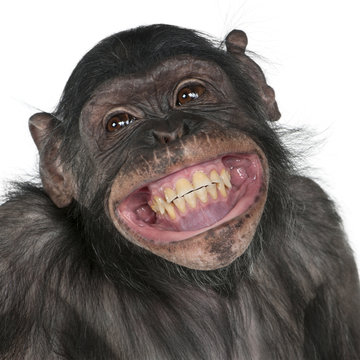
\includegraphics{Pictures/monkey.jpg}
    \label{fig:malpa}


\section{Lista numerowana}
    \begin{enumerate}
    \item Raz
    \item Dwa
\end{enumerate}


\section{Lista nienumerowana}
    \begin{itemize}
     \item Jeden
     \item Dwa
     \end{itemize}

\section{Akapit}

Dotychczas naukowcy zidentyfikowali na całym świecie ponad \textbf{20 gatunków} pasożytniczych grzybów z rodzaju \emph{Ophiocordyceps}. Ich działanie sprawia, że insekty tracą kontrolę nad ciałem i zachowują się jak zombie. Oczywiście cały proces jest \underline{o wiele bardziej skomplikowany}.

To kolejne odkrycie przybliżające do poznania prawdy o insektach uchodzących za najbardziej pracowite w królestwie zwierząt. Nie wszystkie mrówki to robotnice i nie wszystkie gatunki są do siebie podobne. Czy to w wyglądzie, czy w zachowaniu. Przykładowo roślinożerne mrówki mają „zęby” jak noże. To zasługa atomów cynku.




\section{Tabela}
\begin{table}[h!]
\begin{tabular}{lllll}
\cline{1-3}
\multicolumn{1}{|c|}{1} & \multicolumn{1}{c|}{2} & \multicolumn{1}{c|}{3} &  &  \\ \cline{1-3}
\multicolumn{1}{|c|}{6} & \multicolumn{1}{c|}{7} & \multicolumn{1}{c|}{8} &  &  \\ \cline{1-3}
                        &                        &                        &  &  \\
                        &                        &                        &  & 
\end{tabular}
\end{table}




\end{document}